\documentclass{beamer}

\usepackage[orientation=portrait, size=a0, scale=1.4]{beamerposter}

% \usetheme{confposter} % Use the confposter theme supplied with this template

\usepackage[utf8]{inputenc}
\usepackage[T1]{fontenc}
\usepackage[francais]{babel}

\usepackage{graphicx}
\usepackage{subfig}
\usepackage{xcolor}
\usepackage{enumitem}

\definecolor{framebg}{RGB}{225, 225, 225}
\definecolor{titlebg}{RGB}{102, 205, 0}
\definecolor{titleboxbg}{RGB}{50, 205, 50}

\setbeamertemplate{blocks}[rounded][shadow=false]
\setbeamertemplate{caption}[numbered]

\begin{document}
    \setbeamercolor{background canvas}{bg=framebg}
    \begin{frame}[t]
        %---------------------------
        %-          TITLE          -
        %---------------------------

        \setbeamercolor{block body}{fg=black,bg=titlebg} % Colors of the block titles
        \begin{block}{}
            \begin{columns}[t]
                \begin{column}{.1\linewidth}
                    \begin{figure}[t]
                        
\includegraphics[width=\linewidth]{rsc/logo_um.png}
                    \end{figure}
                \end{column}

                \begin{column}{.75\linewidth}
                    \begin{center}
                        {\Huge \textbf{Musée sécurisé en réalité augmentée}}
                    \end{center}

                    \begin{columns}[t]
                        \begin{column}{.5\linewidth}
                            \begin{center}
                                \textbf{Présenté par\\Théo Clayette, Thibaut Etienne, Arnaud Soulier}
                            \end{center}
                        \end{column}

                        \begin{column}{.5\linewidth}
                            \begin{center}
                                \textbf{Sous la direction de\\William Puech, Pauline Puteaux}
                            \end{center}
                        \end{column}
                    \end{columns}
                \end{column}

                \begin{column}{.1\linewidth}
                    \begin{figure}[t]
                        
\includegraphics[width=\linewidth]{rsc/logo_lirmm.png}
                    \end{figure}
                \end{column}
            \end{columns}
        \end{block}

        % \rule{\linewidth}{2mm}

        %----------------------------
        %-          POSTER          -
        %----------------------------

        \begin{columns}[t]
            %------------------------------------------
            %-          POSTER - CHIFFREMENT          -
            %------------------------------------------

            \begin{column}{.49\linewidth}

                %--------------------------------
                %-          C1 - INDEX          -
                %--------------------------------

                \setbeamercolor{block title}{fg=white,bg=titleboxbg} % Colors of the block titles
                \setbeamercolor{block body}{fg=black,bg=white} % Colors of the block titles
                \begin{block}{\centering \textbf{Chiffrement - Méthode}}
                    \vspace{.5cm}

                    \begin{figure}[t]
                        \begin{center}
                            \captionsetup[subfigure]{justification=centering}
                            \subfloat[Itération 1]{
                                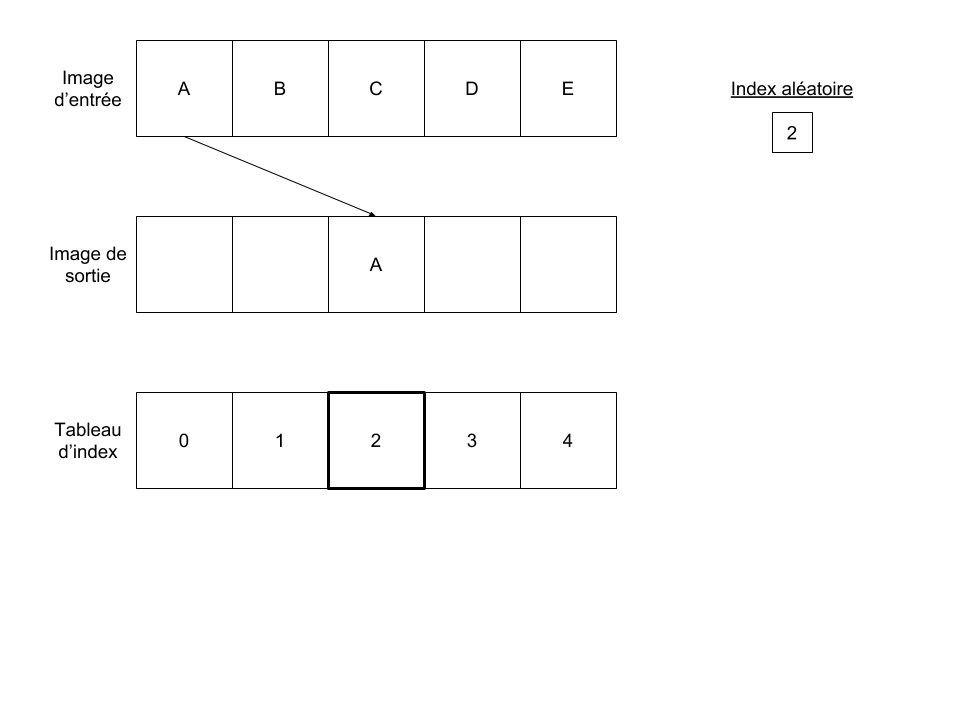
\includegraphics[width=.3\linewidth]{rsc/index_1.png}}
                            \subfloat[Itération 2]{
                                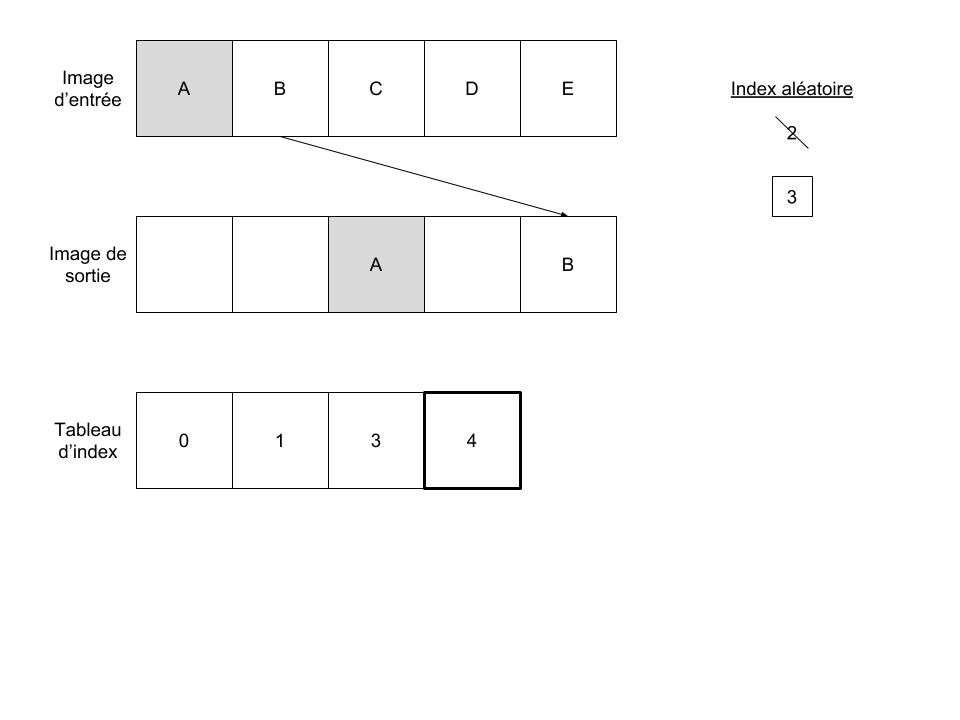
\includegraphics[width=.3\linewidth]{rsc/index_2.png}}
                            \subfloat[Itération 3]{
                                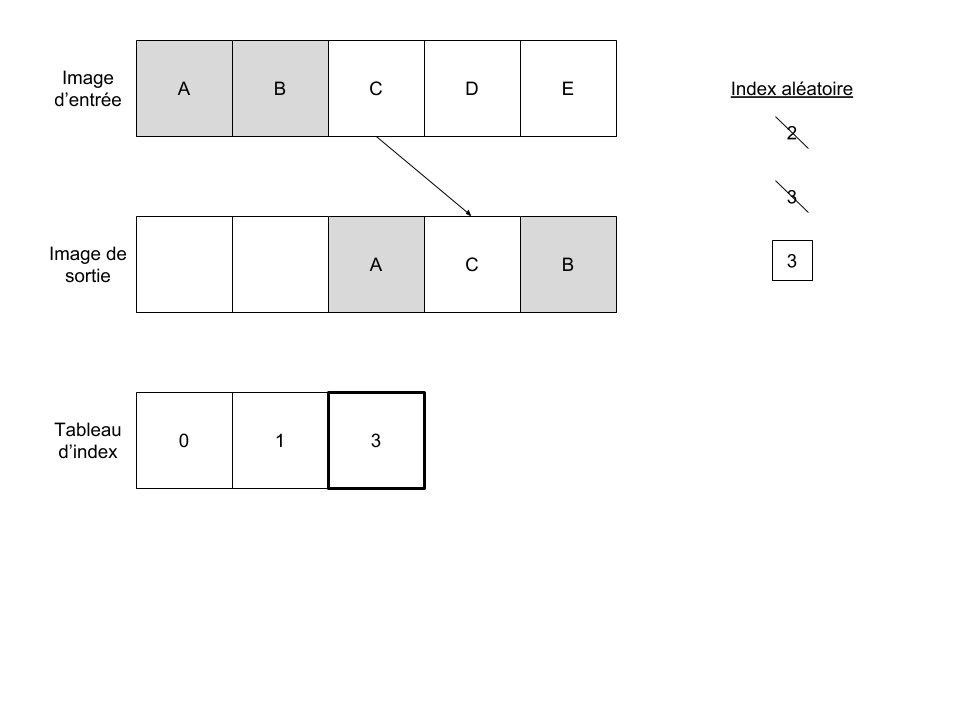
\includegraphics[width=.3\linewidth]{rsc/index_3.png}}
                            \caption{Algorithme de chiffrement pseudo-aléatoire}
                        \end{center}
                    \end{figure}

                    Chaque itération se décompose en 4 étapes :
                    \begin{itemize}[label=-]
                        \item Tirage d'un nombre aléatoire $r$ entre 0 et la taille d'un tableau d'index.
                        \item Récupération du nouvel indice $n$ du pixels dans le tableau d'index à l'indice $r$.
                        \item Écriture du pixels dans la nouvelle case $n$ de l'image de sortie.
                        \item Suppression de la case $n$ du tableau d'index.
                    \end{itemize}

                    \vspace{.5cm}
                \end{block}

                \vspace{.5cm}

                %------------------------------------
                %-          C1 - Résultats          -
                %------------------------------------

                \setbeamercolor{block title}{fg=white,bg=titleboxbg} % Colors of the block titles
                \setbeamercolor{block body}{fg=black,bg=white} % Colors of the block titles
                \begin{block}{\centering \textbf{Chiffrement - Résultats}}
                    \vspace{.5cm}

                    \begin{figure}[t]
                        \begin{center}
                            \captionsetup[subfigure]{justification=centering}
                            \subfloat[Image original de 800x800 pixels]{
                                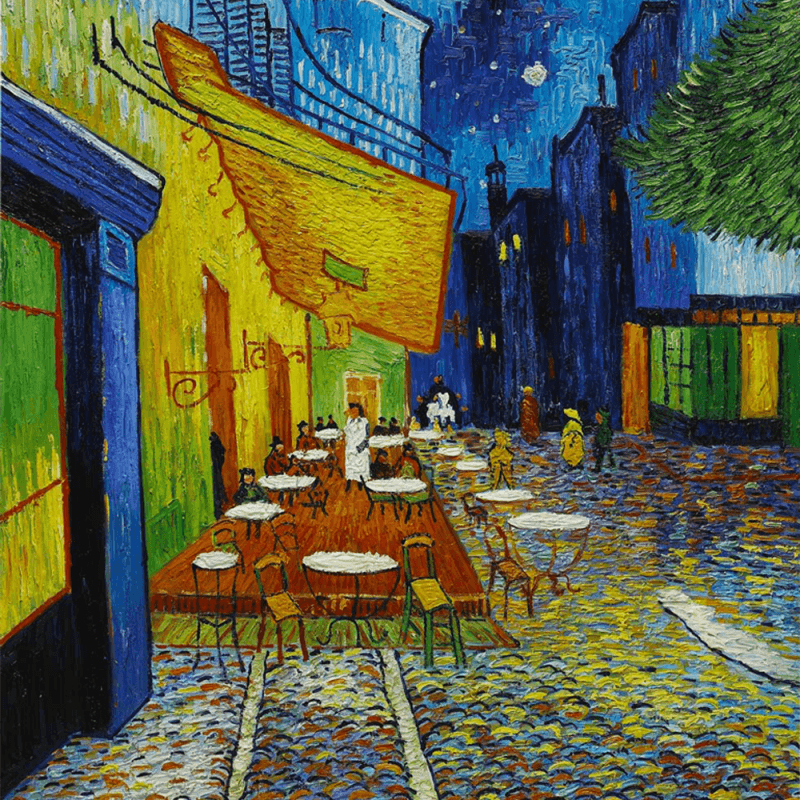
\includegraphics[width=.25\linewidth]{rsc/van_gogh.png}}
                            \hspace{.05\linewidth}
                            \subfloat[Chiffrement par 800x800 blocs de 1x1 pixels]{
                                
\includegraphics[width=.25\linewidth]{rsc/van_gogh_800_12.png}}\\
                            \subfloat[Chiffrement par 10x10 blocs de 80x80 pixels]{
                                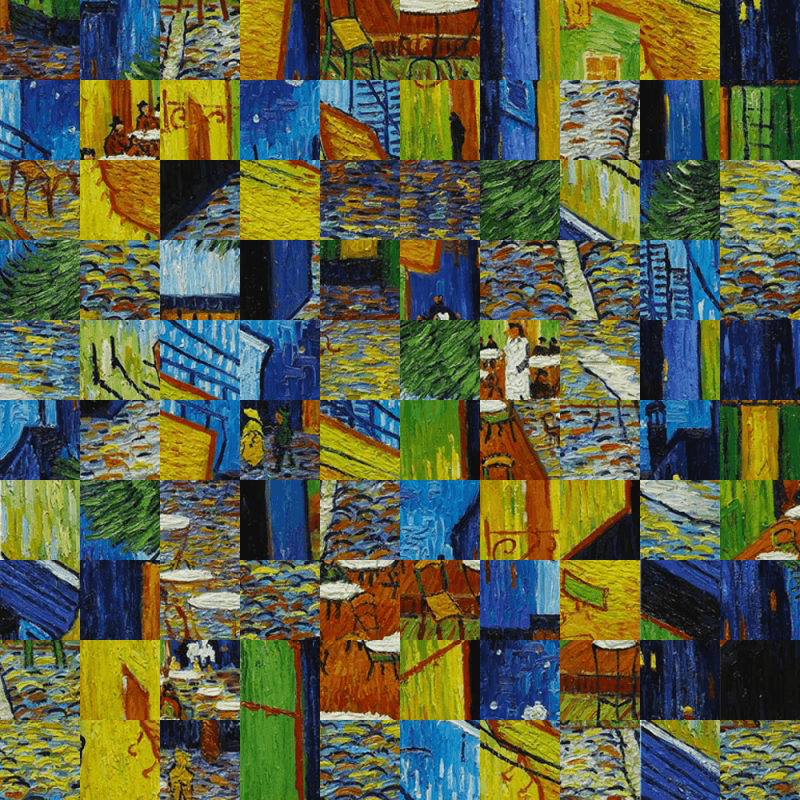
\includegraphics[width=.25\linewidth]{rsc/van_gogh_10_12.png}}
                            \hspace{.05\linewidth}
                            \subfloat[Chiffrement par 25x25 blocs de 32x32 pixels]{
                                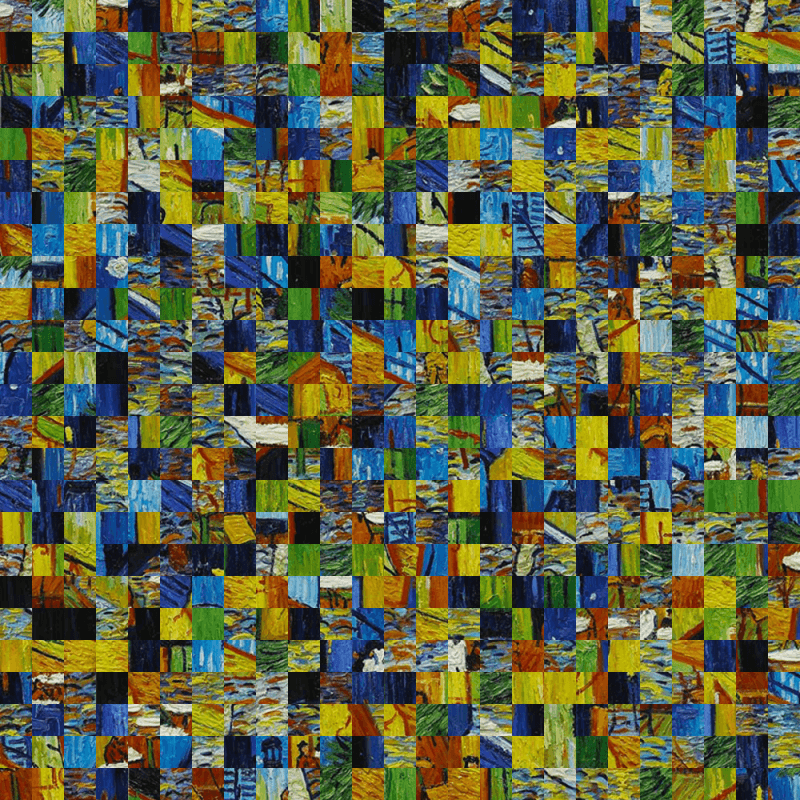
\includegraphics[width=.25\linewidth]{rsc/van_gogh_25_12.png}}
                            \hspace{.05\linewidth}
                            \subfloat[Chiffrement par 50x50 blocs de 16x16 pixels]{
                                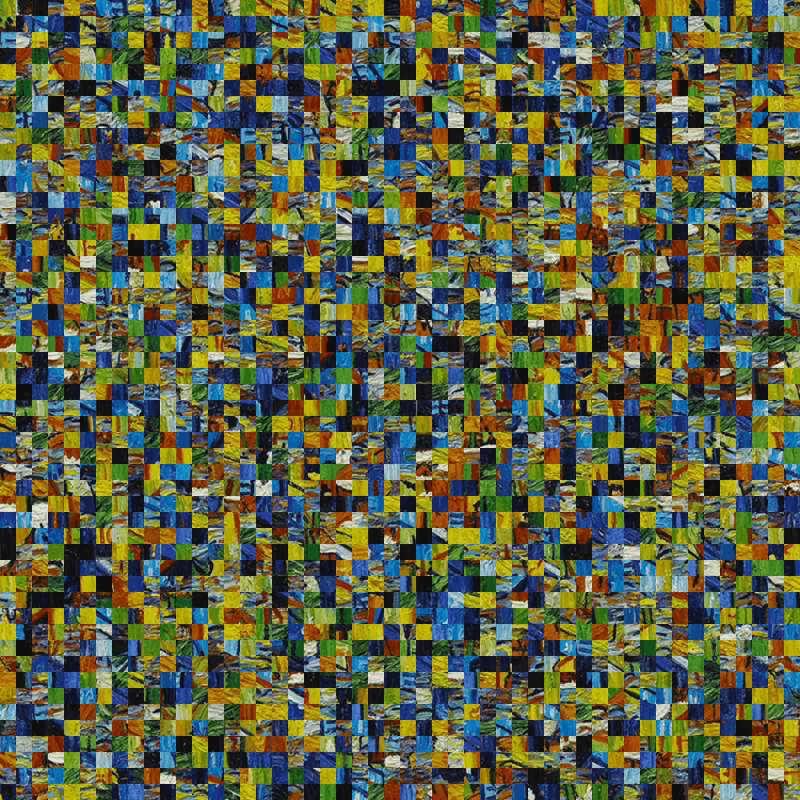
\includegraphics[width=.25\linewidth]{rsc/van_gogh_50_12.png}}\\
                            \subfloat[Chiffrement par 10x10 blocs de 80x80 pixels moyennés]{
                                
\includegraphics[width=.25\linewidth]{rsc/van_gogh_a_10_12.png}}
                            \hspace{.05\linewidth}
                            \subfloat[Chiffrement par 25x25 blocs de 32x32 pixels moyennés]{
                                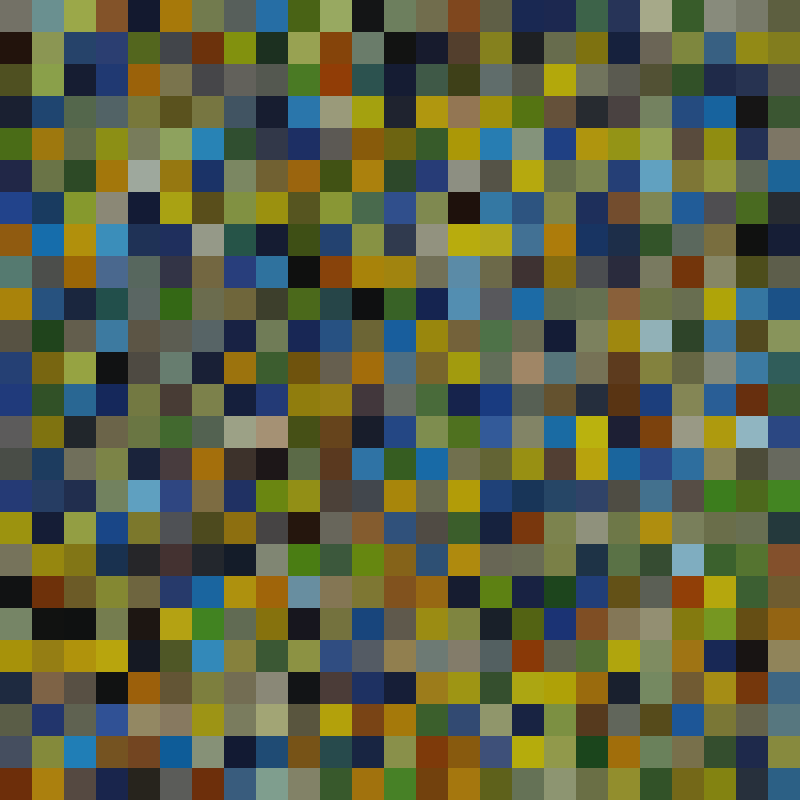
\includegraphics[width=.25\linewidth]{rsc/van_gogh_a_25_12.png}}
                            \hspace{.05\linewidth}
                            \subfloat[Chiffrement par 50x50 blocs de 16x16 pixels moyennés]{
                                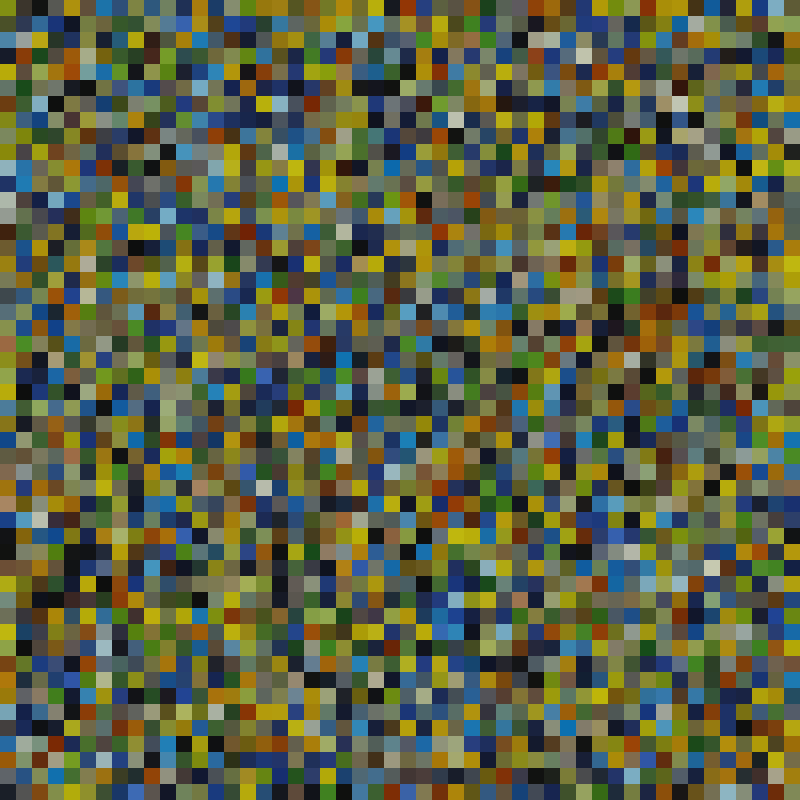
\includegraphics[width=.25\linewidth]{rsc/van_gogh_a_50_12.png}}\\
                            \caption{Chiffrement par bloc et bloc moyenné de l'oeuvre "Térasse du café le soir" de Van Gogh}
                        \end{center}
                    \end{figure}
                \end{block}

                \vspace{.5cm}

                %-----------------------------------------------
                %-          C2 - QUALITE RESSEMBLANCE          -
                %-----------------------------------------------

                \setbeamercolor{block title}{fg=white,bg=titleboxbg} % Colors of the block titles
                \setbeamercolor{block body}{fg=black,bg=white} % Colors of the block titles
                \begin{block}{\centering \textbf{Qualité de ressemblance de l'oeuvre}}
                    \vspace{.5cm}

                    \begin{center}
                        \begin{figure}[t]
                            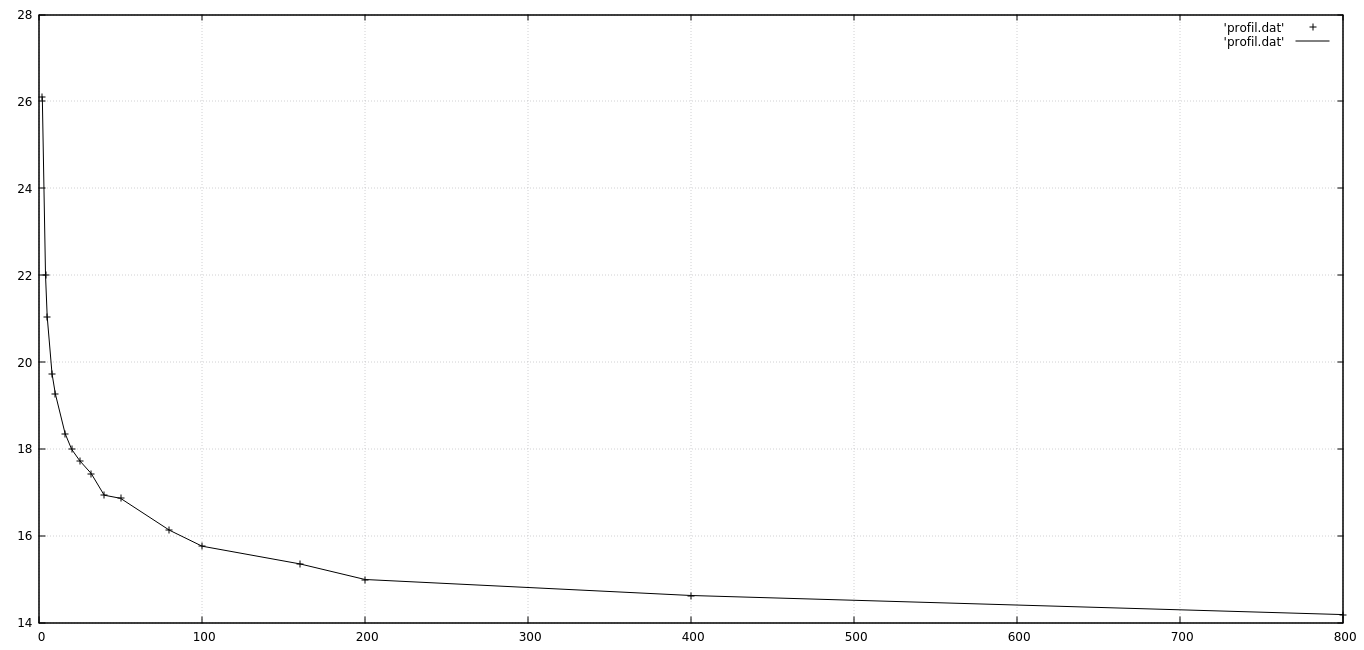
\includegraphics[width=.5\linewidth]{rsc/psnr_ressemblance.png}
                            \caption{PSNR de la peinture en fonction de la taille des blocs}
                        \end{figure}
                    \end{center}

                    D'après le PSNR (Peak Signal to Noise Ratio) obtenu avec le découpage en bloc de diverses tailles de la peinture, on observe une qualité acceptable (PSNR >= 20 db) à partir d'une taille de bloc de 8x8 pixels (19.6387 db).
                    Toutes les décompositions avec des blocs d'une taille inférieure ou égale à 8x8 pixels sont considéré comme ressemblante à l'oeuvre d'origine.

                    \vspace{.5cm}
                \end{block}

                \vspace{.5cm}

                %----------------------------------------
                %-          C2 - PRETRAITEMENT          -
                %----------------------------------------

                \setbeamercolor{block title}{fg=white,bg=titleboxbg} % Colors of the block titles
                \setbeamercolor{block body}{fg=black,bg=white} % Colors of the block titles
                \begin{block}{\centering \textbf{Lecture - Prétraitements}}
                    \vspace{.5cm}

                    Traitement à effectuer sur la photo pour permettre la transformation :
                    \begin{itemize}[label=\textbullet]
                        \item Conversion en image en niveau de gris :
                        \begin{itemize}[label=$\rightarrow$]
                            \item 0.299 $\cdot$ rouge + 0.587 $\cdot$ vert + 0.114 $\cdot$ bleu.
                        \end{itemize}
                        \item Conversion en image binaire :
                        \begin{itemize}[label=$\rightarrow$]
                            \item sépare la peinture du fond pour failiter la détection des angles.
                            \item utilise la variance moyenne comme valeur de seuil
                        \end{itemize}
                        \item Détection des angles :
                        \begin{itemize}[label=$\rightarrow$]
                            \item trouve les quatres points tels que leurs distances aux coins respectifs de l'image soit minimale.
                        \end{itemize}
                    \end{itemize}

                    \vspace{.5cm}
                \end{block}
            \end{column}

            %--------------------------------------------
            %-          POSTER - DECHIFFREMENT          -
            %--------------------------------------------

            \begin{column}{.49\linewidth}

                %----------------------------------------
                %-          C2 - TRANFORMATION          -
                %----------------------------------------

                \setbeamercolor{block title}{fg=white,bg=titleboxbg} % Colors of the block titles
                \setbeamercolor{block body}{fg=blue,bg=white} % Colors of the block titles
                \begin{block}{\centering \textbf{Lecture - Transformation}}
                    \begin{figure}[t]
                        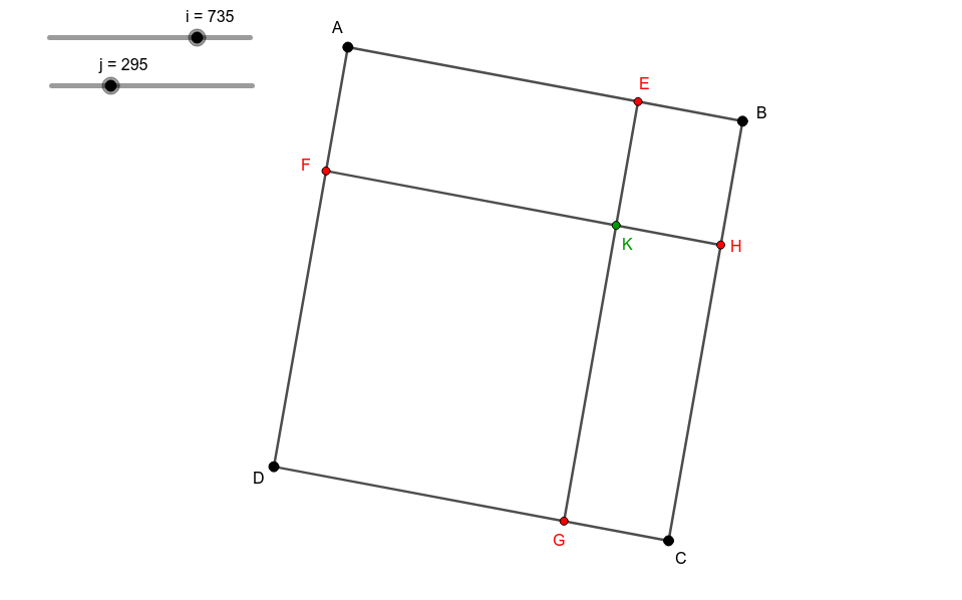
\includegraphics[width=.5\linewidth]{rsc/formule_transformation.png}\\
                    \end{figure}
                \end{block}

                \vspace{1cm}

                %------------------------------------
                %-          C2 - RESULTATS          -
                %------------------------------------

                \setbeamercolor{block title}{fg=white,bg=titleboxbg} % Colors of the block titles
                \setbeamercolor{block body}{fg=black,bg=white} % Colors of the block titles
                \begin{block}{\centering \textbf{Lecture - Résultats}}
                    \begin{columns}[t]
                        \begin{column}{.2\linewidth}
                            \begin{figure}[t]
                                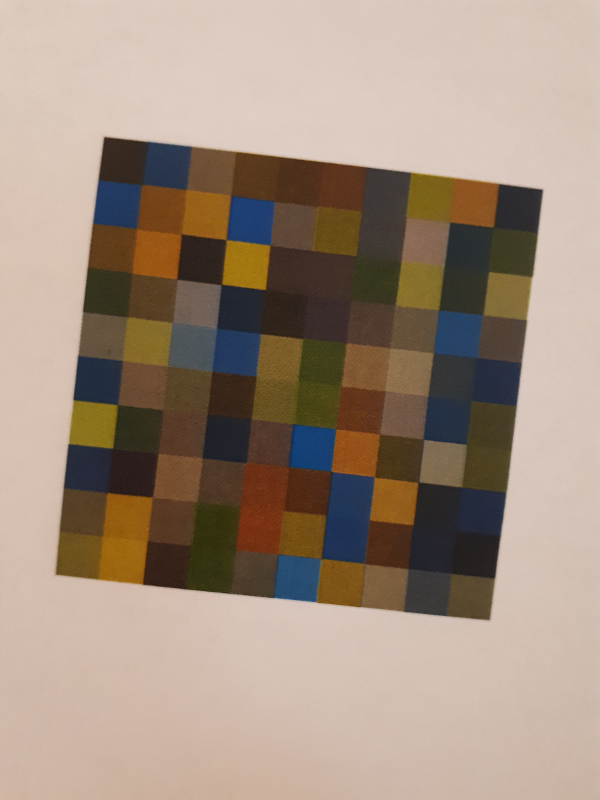
\includegraphics[width=\linewidth]{rsc/van_gogh_picture_a_10.png}\\
                            \end{figure}
                        \end{column}

                        \begin{column}{.2\linewidth}
                            \begin{figure}[t]
                                \hspace{.5cm}
                                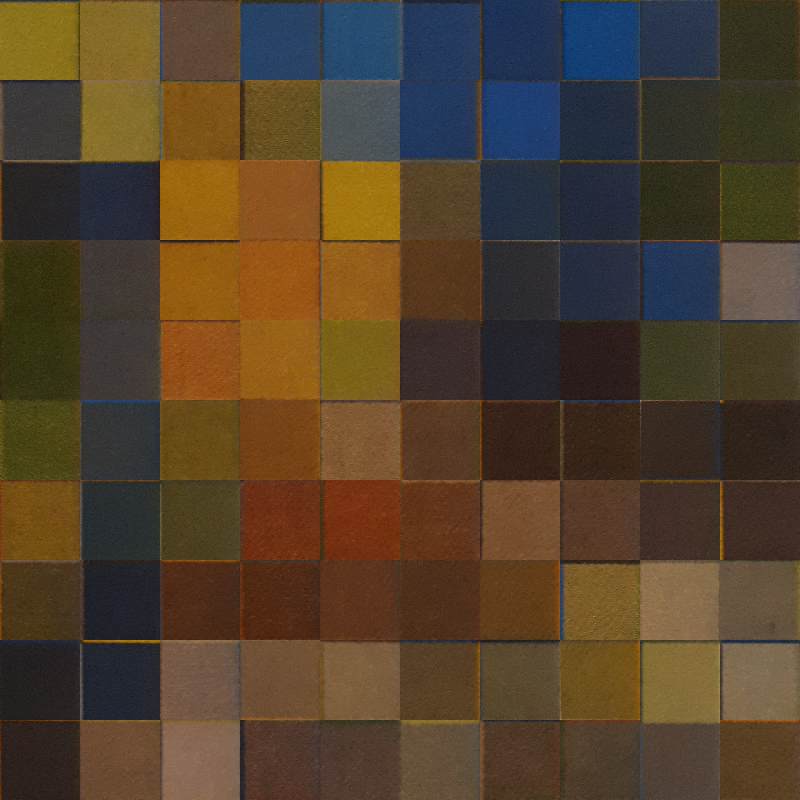
\includegraphics[width=\linewidth]{rsc/van_gogh_picture_a_10_d.png}\\
                            \end{figure}
                        \end{column}

                        \begin{column}{.005\linewidth}

                        \end{column}

                        \begin{column}{.2\linewidth}
                            \begin{figure}[t]
                                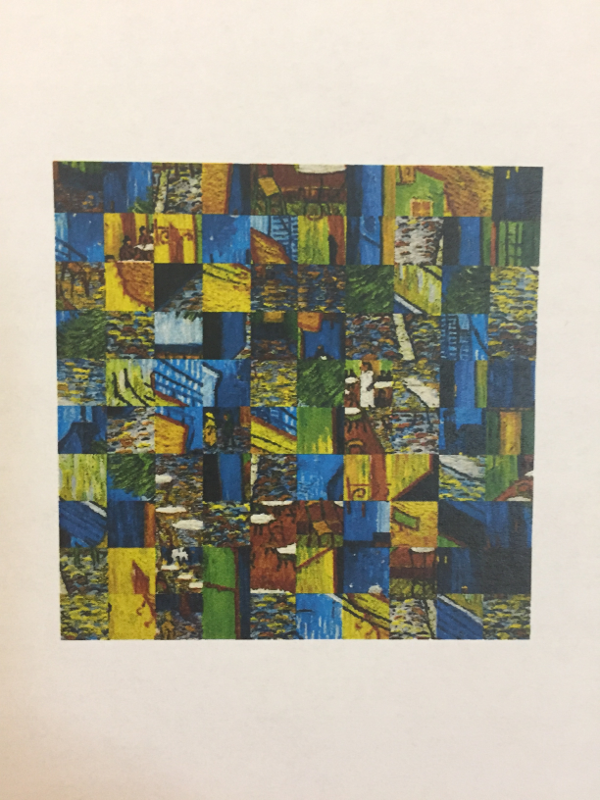
\includegraphics[width=\linewidth]{rsc/van_gogh_picture_10.png}\\
                            \end{figure}
                        \end{column}

                        \begin{column}{.2\linewidth}
                            \begin{figure}[t]
                                \hspace{.5cm}
                                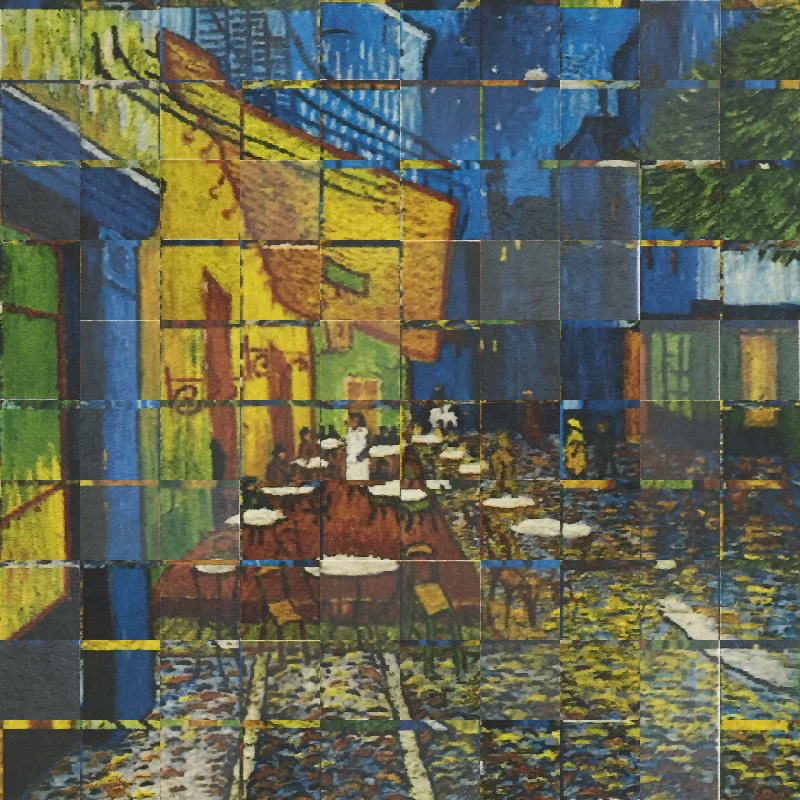
\includegraphics[width=\linewidth]{rsc/van_gogh_picture_10_d.png}\\
                            \end{figure}
                        \end{column}
                    \end{columns}

                    \begin{columns}[t]
                        \begin{column}{.5\linewidth}
                            \begin{center}
                                {\small Déchiffrement 10x10 blocs de 80x80 pixels moyennés}
                            \end{center}
                        \end{column}

                        \begin{column}{.5\linewidth}
                            \begin{center}
                                {\small Déchiffrement 10x10 blocs de 80x80 pixels}
                            \end{center}
                        \end{column}
                    \end{columns}

                    \begin{figure}[t]
                        \begin{center}
                            \captionsetup[subfigure]{justification=centering}
                            \subfloat[Photo 80x80 pixels]{
                                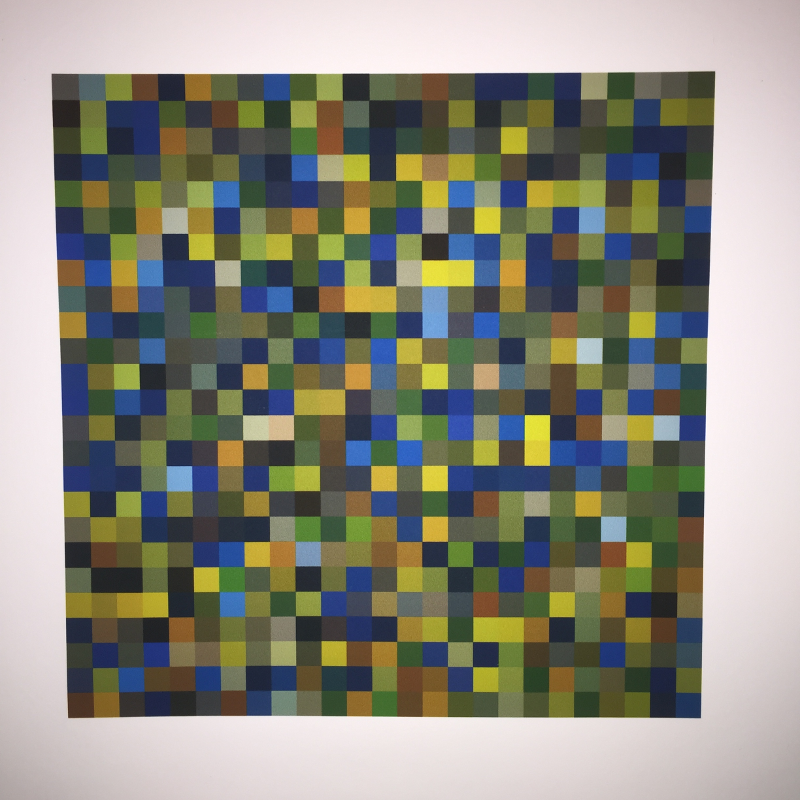
\includegraphics[width=.25\linewidth]{rsc/van_gogh_25.png}}
                            \hspace{.05\linewidth}
                            \subfloat[Photo 32x32 pixels]{
                                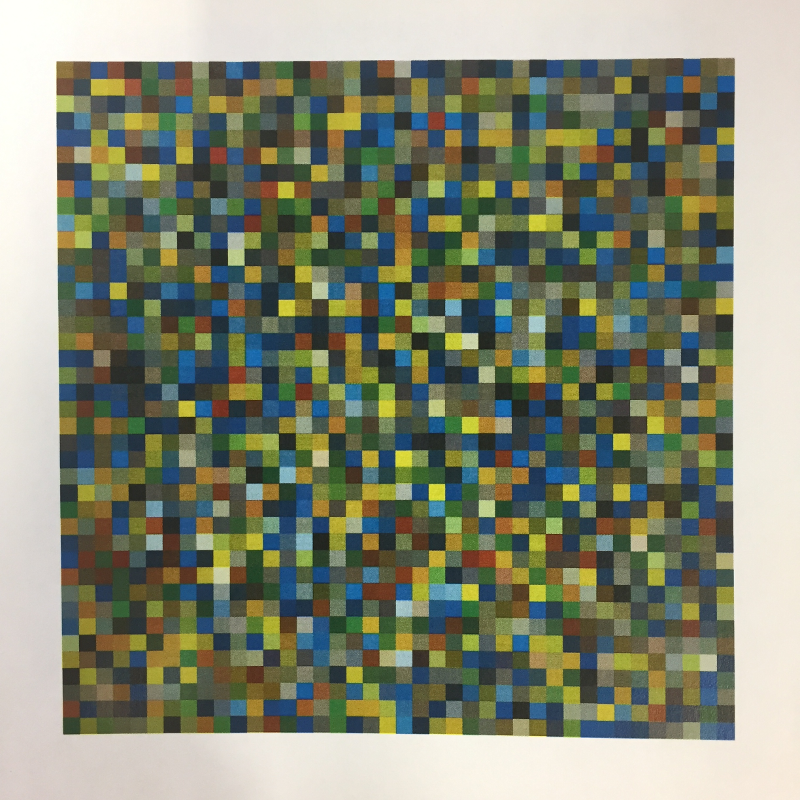
\includegraphics[width=.25\linewidth]{rsc/van_gogh_40.png}}
                            \hspace{.05\linewidth}
                            \subfloat[Photo 16x16 pixels]{
                                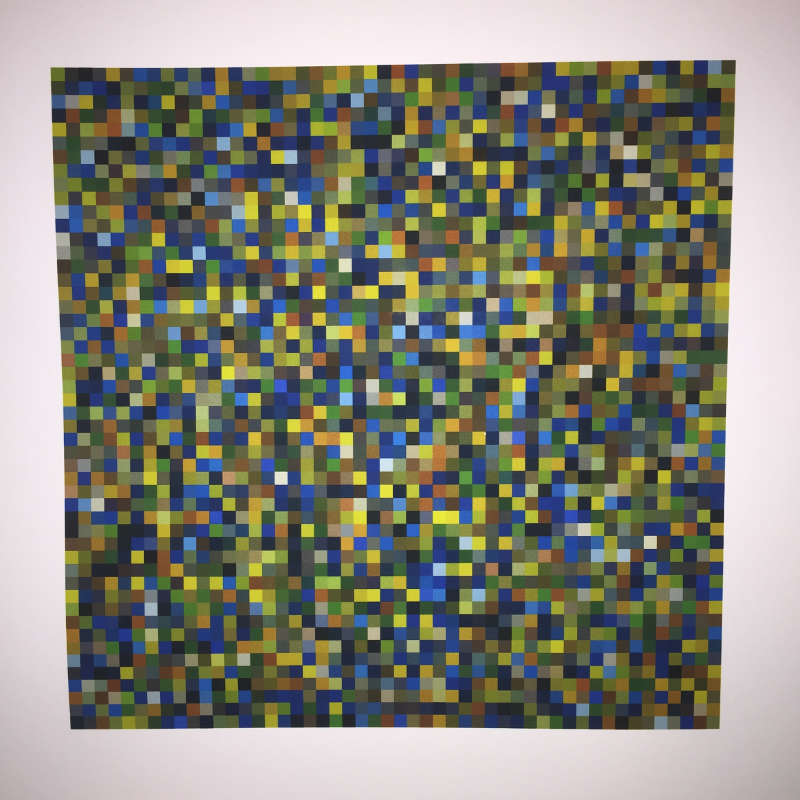
\includegraphics[width=.25\linewidth]{rsc/van_gogh_50.png}}\\
                            \subfloat[Déchiffrement 80x80 pixels]{
                                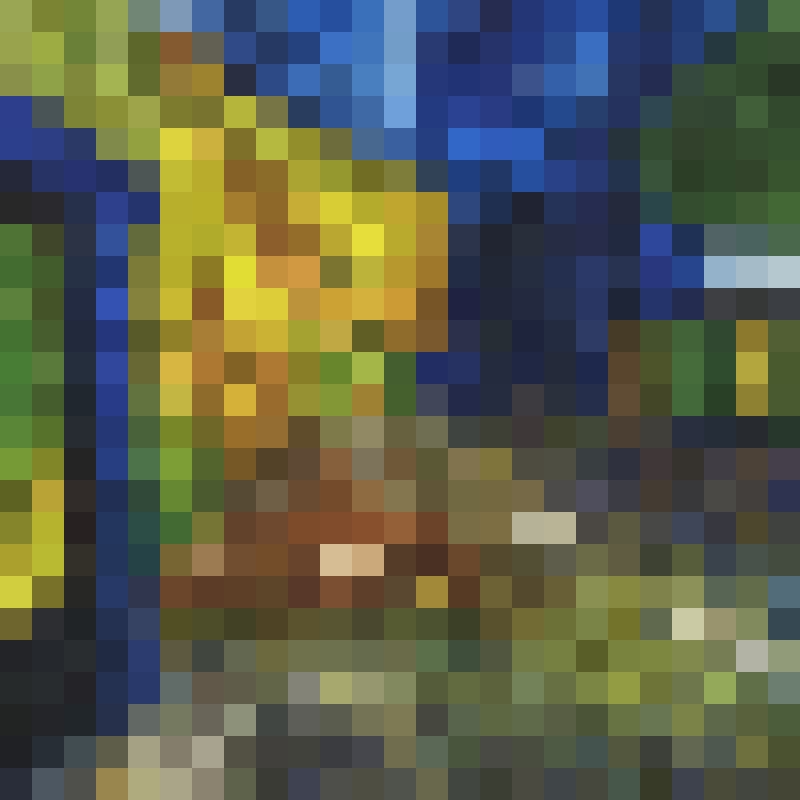
\includegraphics[width=.25\linewidth]{rsc/van_gogh_25_d_a.png}}
                            \hspace{.05\linewidth}
                            \subfloat[Déchiffrement 32x32 pixels]{
                                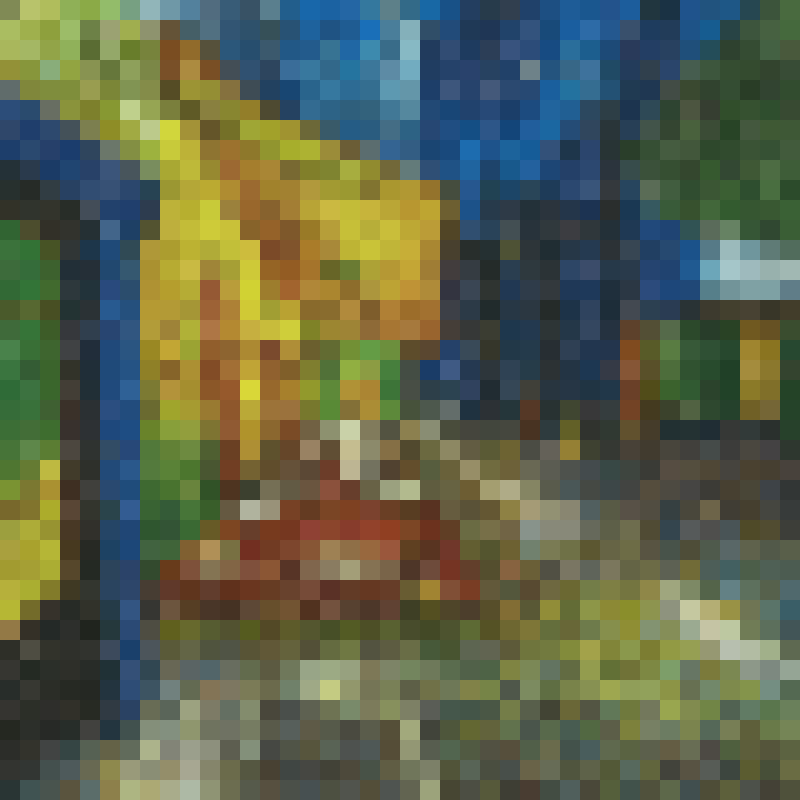
\includegraphics[width=.25\linewidth]{rsc/van_gogh_40_d_a.png}}
                            \hspace{.05\linewidth}
                            \subfloat[Déchiffrement 16x16 pixels]{
                                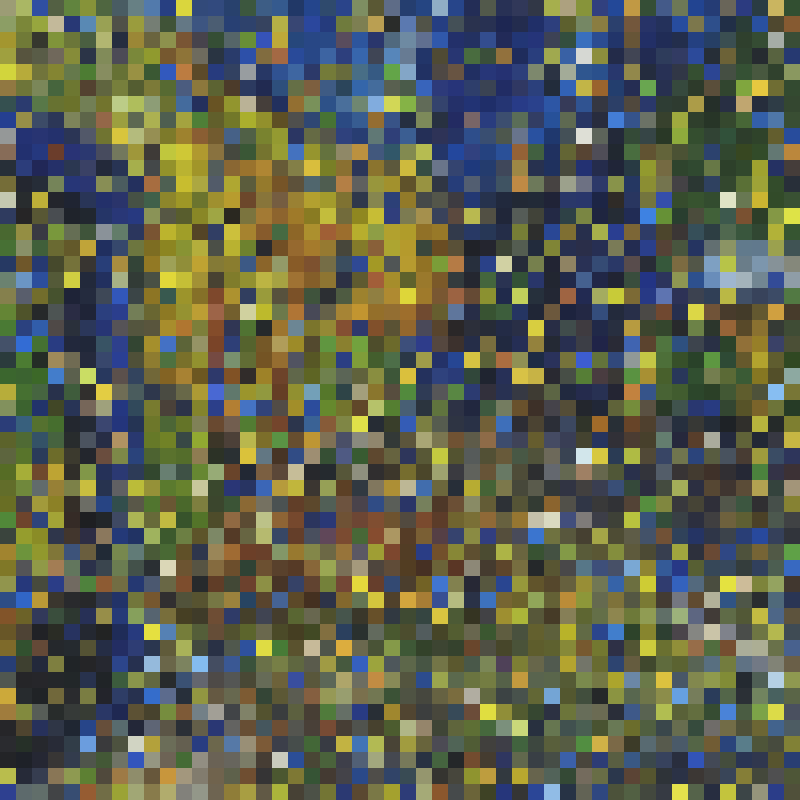
\includegraphics[width=.25\linewidth]{rsc/van_gogh_50_d_a.png}}\\
                            \caption{Lecture et déchiffrement par bloc moyenné de l'oeuvre "Térasse du café le soir" de Van Gogh}
                        \end{center}
                    \end{figure}
                \end{block}

                \vspace{1cm}

                %------------------------------------------
                %-          C2 - QUALITE LECTURE          -
                %------------------------------------------

                \setbeamercolor{block title}{fg=white,bg=titleboxbg} % Colors of the block titles
                \setbeamercolor{block body}{fg=black,bg=white} % Colors of the block titles
                \begin{block}{\centering \textbf{Qualité de lecture de l'oeuvre imprimée}}
                    \begin{center}
                        \begin{figure}[t]
                            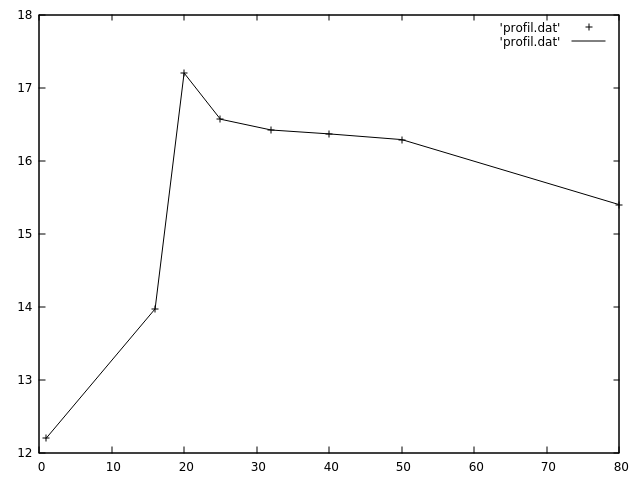
\includegraphics[width=.5\linewidth]{rsc/psnr_lecture.png}
                            \caption{PSNR de la lecture de la peinture en fonction de la taille des blocs}
                        \end{figure}
                    \end{center}

                    La qualité d'acquisition de l'image dépend de l'appareil utilisé. Dans le cadre de ce projet, il s'agit d'une Iphone 6.
                    Plus la taille des blocs est petite, plus la peinture déchiffré est ressemblante à l'oeuvre d'origine. Cependant, si l'on atteint la taille de 16x16 pixels, la précision de l'image est trop faible pour permettre un déchiffrement correct de la peinture.
                    Le meilleur résultat obtenable avec cet appareil est avec un découpage en blocs de maximum 20x20 pixels.
                \end{block}
            \end{column}
        \end{columns}
    \end{frame}
\end{document}
